\begin{figure}[!ht]
    \centering
    \begin{tabular}[c]{ccc}
    \begin{subfigure}[c]{0.31\textwidth}
        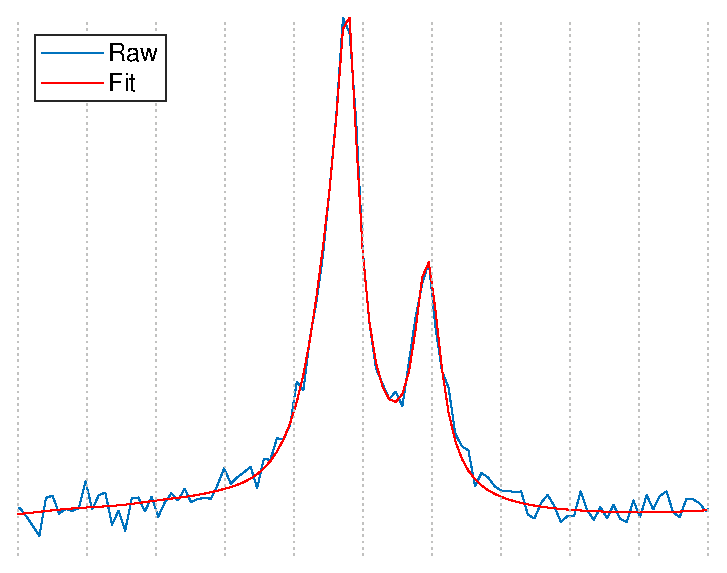
\includegraphics[width=0.95\textwidth,keepaspectratio]{images/b0_peaks/no_B0.eps}
        \caption{Spectral peaks without $B_0$ inhomogeneities ($\mu = 0$Hz)}
        \label{subfig:without B0}
        \vspace{3pt}
    \end{subfigure}&
    \begin{subfigure}[c]{0.31\textwidth}
        \centering
        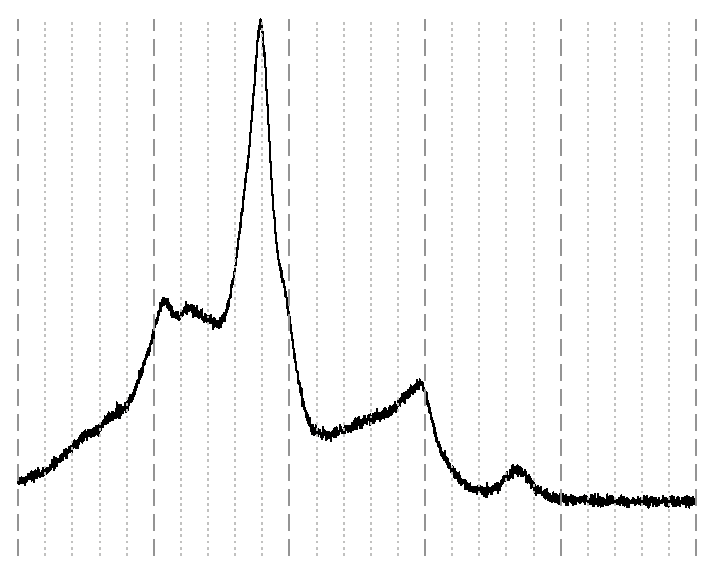
\includegraphics[width=0.95\textwidth,keepaspectratio]{images/b0_peaks/some_B0.eps}
        \caption{Spectral peaks with moderate $B_0$ inhomogeneities ($\mu = 75$Hz)}
        \label{subfig:some B0}      
        \vspace{3pt}
    \end{subfigure}&
    \begin{subfigure}[c]{0.31\textwidth}
        \centering
        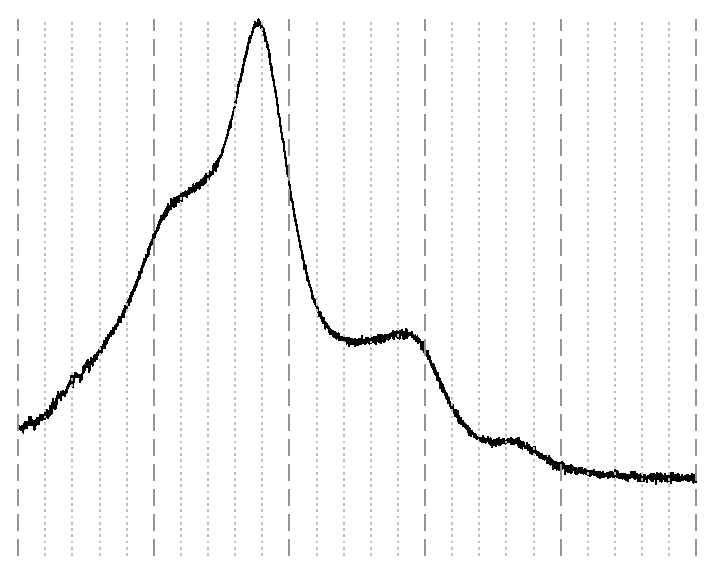
\includegraphics[width=0.95\textwidth,keepaspectratio]{images/b0_peaks/with_B0.eps}
        \caption{Spectral peaks with severe $B_0$ inhomogeneities ($\mu = 175$Hz)}
        \label{subfig:with B0}  
        \vspace{3pt}
    \end{subfigure}\\
    \begin{subfigure}[c]{0.31\textwidth}
        \centering
        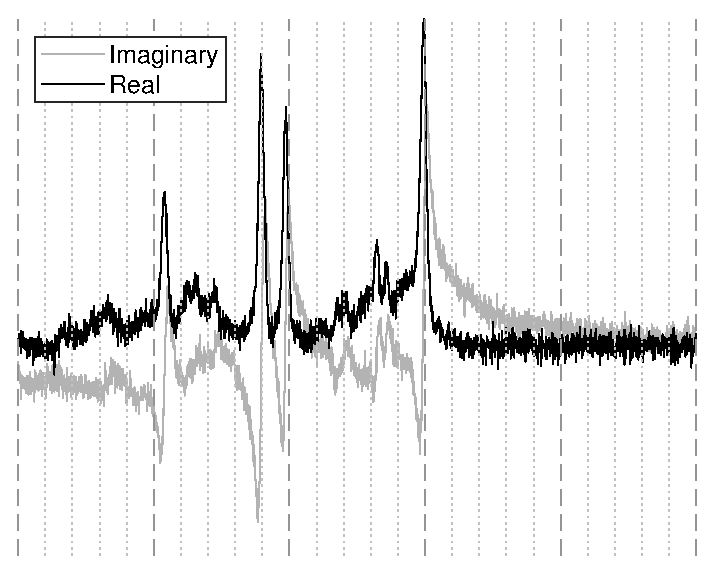
\includegraphics[width=0.95\textwidth,keepaspectratio]{images/phase/no_phase.eps}
        \caption{Spectrum with no phase offsets}
        \label{subfig:no phase}        
        \vspace{3pt}
    \end{subfigure}&
    \begin{subfigure}[c]{0.31\textwidth}
        \centering
        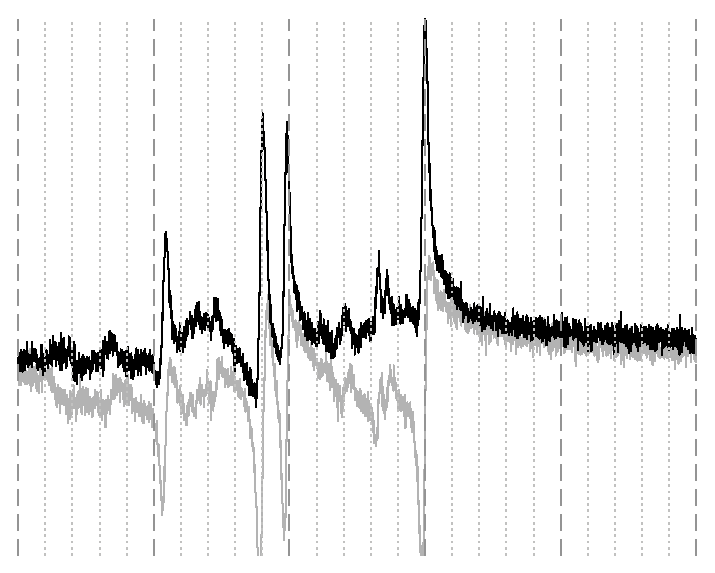
\includegraphics[width=0.95\textwidth,keepaspectratio]{images/phase/zero-order.eps}
        \caption{Spectrum with zero-order phase offset ($\phi_0 = 45^{\circ}$)}
        \label{subfig:zero order phase}        
        \vspace{3pt}
    \end{subfigure}&%
    \begin{subfigure}[c]{0.31\textwidth}
        \centering
        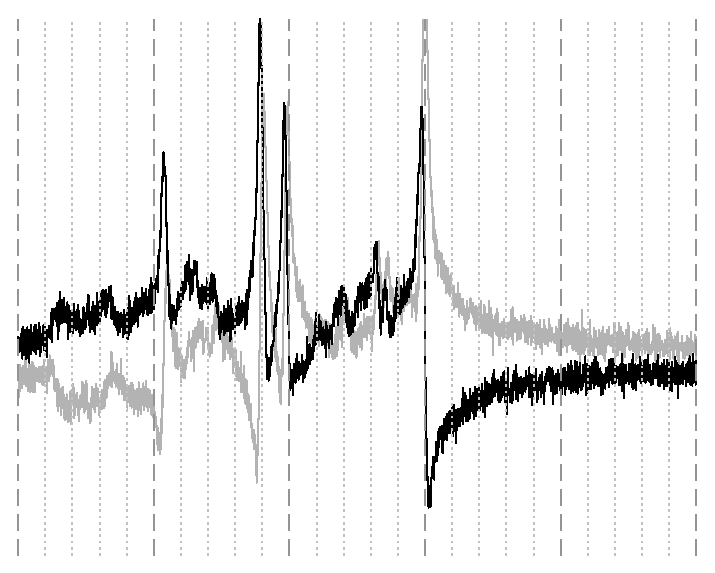
\includegraphics[width=0.95\textwidth,keepaspectratio]{images/phase/first-order.eps}
        \caption{Spectrum with first-order phase offset ($\phi_1 = 20^{\circ}$)}
        \label{subfig:first order phase}        
        \vspace{3pt}
    \end{subfigure}\\
    \begin{subfigure}[c]{0.31\textwidth}
        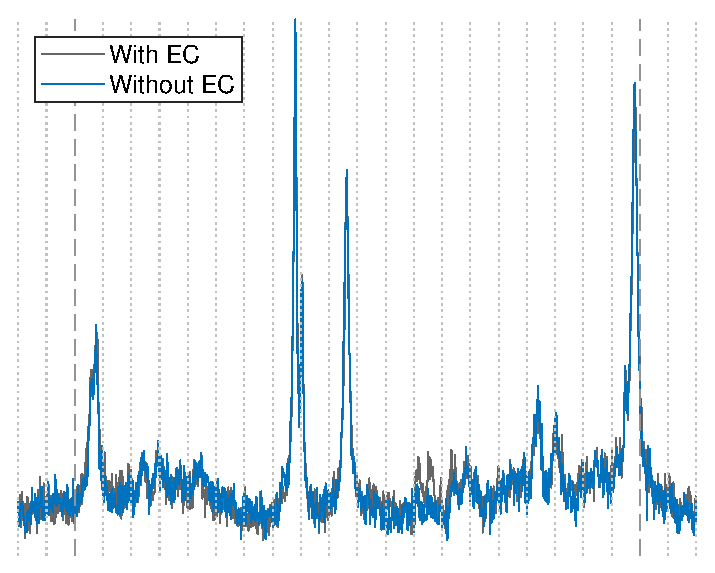
\includegraphics[width=0.95\textwidth, keepaspectratio]{images/eddy/ec=1.eps}
        \caption{Eddy current amplitude = 1.0}
        \label{subfig:ec=1}        
        \vspace{3pt}
    \end{subfigure}&
    \begin{subfigure}[c]{0.31\textwidth}
        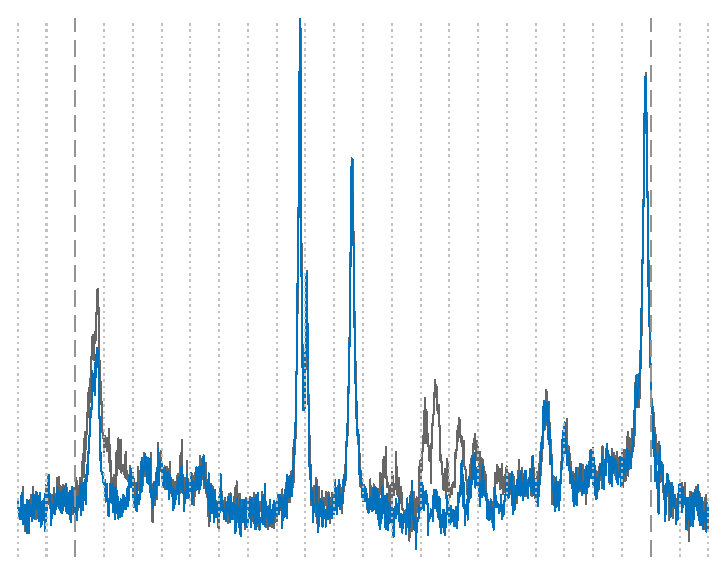
\includegraphics[width=0.95\textwidth, keepaspectratio]{images/eddy/ec=3.eps}
        \caption{Eddy current amplitude = 3.0}
        \label{subfig:ec=3}        
        \vspace{3pt}
    \end{subfigure}&
    \begin{subfigure}[c]{0.31\textwidth}
        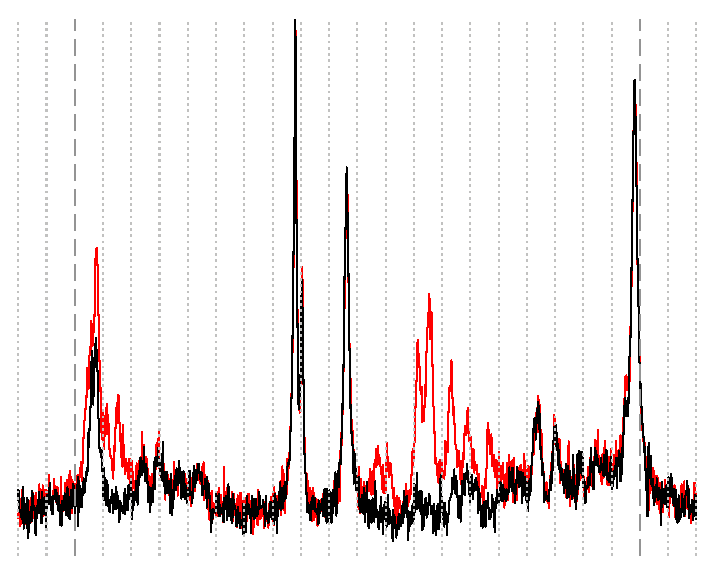
\includegraphics[width=0.95\textwidth, keepaspectratio]{images/eddy/ec=5.eps}
        \caption{Eddy current amplitude = 5.0}
        \vspace{3pt}
    \end{subfigure}\\
    \begin{subfigure}[c]{0.31\textwidth}
        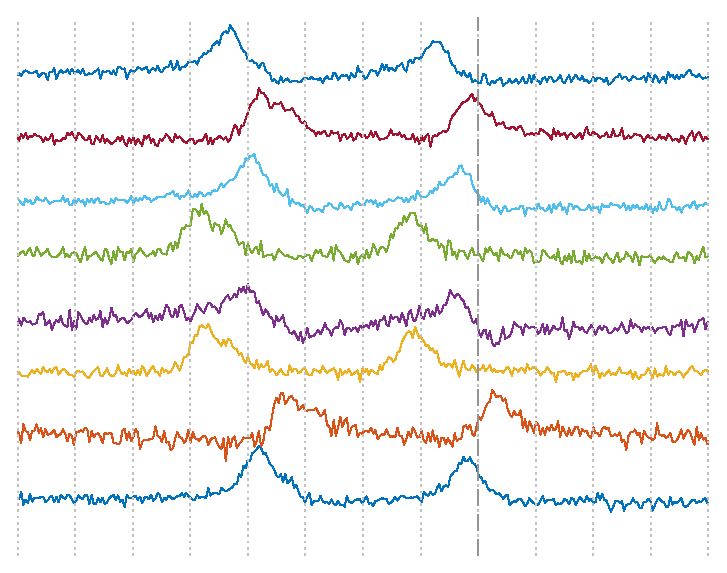
\includegraphics[width=0.95\textwidth, keepaspectratio]{images/samples_transients/8coil_w_phase_w_fshift_cropped.eps}
        \caption{Raw spectral transients}
        \label{subfig:raw transients}      
        \vspace{3pt}
    \end{subfigure}&
    \begin{subfigure}[c]{0.31\textwidth}
        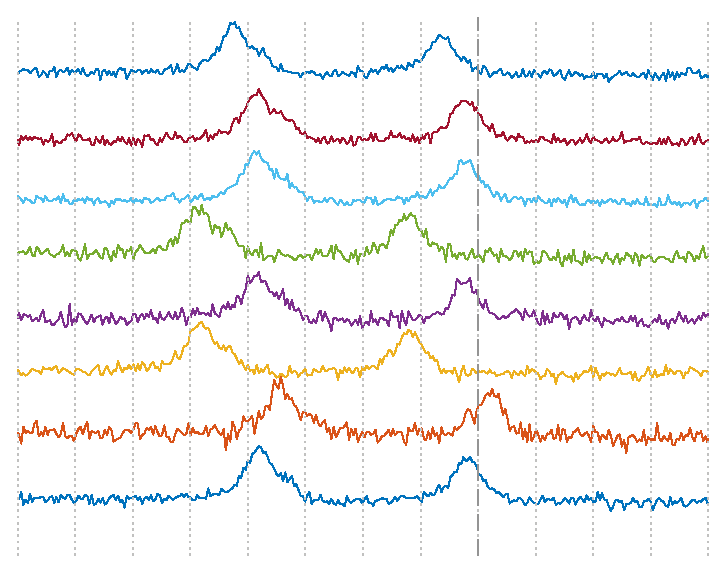
\includegraphics[width=0.95\textwidth, keepaspectratio]{images/samples_transients/8coil_wo_phase_w_fshift_cropped.eps}
        \caption{Phase alignment}
        \label{subfig:phase alignment}        
        \vspace{3pt}
    \end{subfigure}&%
    \begin{subfigure}[c]{0.31\textwidth}
        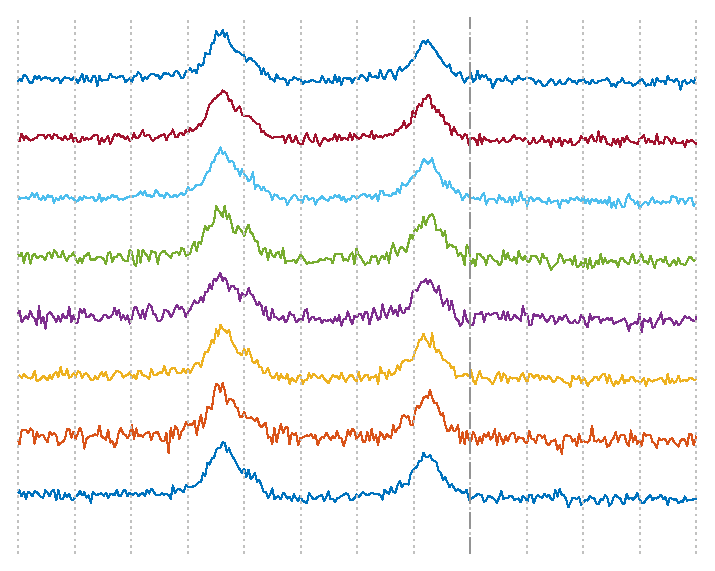
\includegraphics[width=0.95\textwidth, keepaspectratio]{images/samples_transients/8coil_wo_phase_wo_fshift_cropped.eps}
        \caption{Frequency alignment}
        \label{subfig:frequency alignment}      
        \vspace{3pt}
    \end{subfigure}
    \end{tabular}
    \caption{Sample spectra simulated for a PRESS sequence with TE=30ms that highlight the effect of the baseline and residual water contributions.}
    \label{fig:30ms samples curated clean}
\end{figure}
